\chapter[On Upbringing]{Book I On Upbringing and the Life's Condition}

\begin{quote}
\textsl{In the name of God, the merciful and compassionate. May the lord be rich in compassion towards you.}

\textsl{This is the first book of Dorotheus the Egyptian, on the judgments concerning nativities. He chose it and selected it and picked it from the books which were before him, and he wrote it for his son Hermes.}

\textsl{He said to his son at the tie of his testament: I shall relate to you, oh my son, and I shall explain to you so that you may depend on and be confident in your heart about what I shall show you of my work and words according to the stars which indicate for men what will pertain to them from the time of a [person's] birth till his leaving the world, if God wills. I have traveled, o my son, in many cities, and I have seen the wondrous things which are in Egypt and in Babylon, which is in the direction of the Euphrates. I collected the best of their sayings from the first [authorities] who were before me like the bees which gather [honey] from the trees and all kinds of plants; for from it there is the honey of medicine.}
\end{quote}

% Section 1 of Book 1

\section{Triplicity and Sign Rulers}

Know the longitude and latitudes of the seven planets (\Sun,\Moon,\Mercury,\Venus\,\Mars,\Jupiter,\Saturn), the degrees of the Ascendant and MC, which signs are straight and crooked\footnote{The \textsl{straight} signs are those that appear to rise straight up from the horizon taking slightly more than two hours each: \Cancer\, thru \Sagittarius, the remaining signs are called \textsl{crooked} as they rise at an oblique angle to the horizon and each take slightly less than two hours.} in rising, and that the signs, their triplicities and rulers are:

\begin{table}[ht]
\center
\begin{tabular}{| c | c ||  c | c |}
\Xhline{2pt}
\textbf{Sign} & \textbf{Ruler} & \textbf{Sign} & \textbf{Ruler} \\
\hline
\Aries & \Mars & \Libra & \Venus \\ 
\cellcolor{yellow!50!white}\Taurus & \Venus 
	& \cellcolor{yellow!50!white}\Scorpio & \Mars \\ 
\Gemini & \Mercury & \cellcolor{yellow!50!white}\Sagittarius &  \Jupiter \\ 
\Cancer & \Moon & \Capricorn & \Saturn \\ 
\Leo & \Sun & \cellcolor{yellow!50!white}\Aquarius & \Saturn \\ 
\cellcolor{yellow!50!white}\Virgo & \Mercury & \Pisces & \Jupiter \\ 
\hline
\end{tabular}
\caption{Signs and their Domicile Rulers}
\end{table}

The shaded cells represent the sign the planet ruler \textsl{rejoices} or is \textsl{happiest} in.

\begin{table}[ht]
\small
\center
\begin{tabular}{|l | c | c | c |}
\Xhline{2pt}
\textbf{Triplicity} & \multicolumn{3}{c|}{\textbf{Rulers}} \\
 \cline{2-4}
	 & \textbf{Diurnal} & \textbf{Nocturnal} & \textbf{Participating} \\
\hline
\Aries-\Leo-\Sagittarius & \Sun & \Jupiter & \Saturn \\
\Taurus-\Virgo-\Capricorn & \Venus & \Moon & \Mars (and \Mercury\, in \Virgo) \\
\Gemini-\Libra-\Aquarius & \Saturn & \Mercury & \Jupiter \\
\Cancer-\Scorpio-\Pisces & \Venus & \Mars & \Moon \\
\hline
\end{tabular}
\caption{Signs, their Triplicities and Rulers}
\end{table}

The rulers of the triplicities give indications for, and decide, everything.

\begin{mdframed}[backgroundcolor=cyan!5, rightmargin=1em, leftmargin=1em]
\footnotesize
The masculine, diurnal signs are the \Aries-\Leo-\Sagittarius\, and \Gemini-\Libra-\Aquarius\, triplicities and the diurnal planets are \Sun, \Jupiter, and \Saturn.

The feminine, nocturnal signs are the \Taurus-\Virgo-\Capricorn\, and \Cancer-\Scorpio-\Pisces\, triplicities and the nocturnal planets are the \Moon, \Venus, and \Mars\, (with \Mercury\, having a share in \Virgo).

Dorotheus doesn't spell this out until \S{1.28} but in latter sections the reader is assumed to understand these categories.
\end{mdframed}

In mundane astrology, the ``afflictions and distress'' that effect the world are timed and indicated by the triplicity rulers of a solar or lunar eclipse. Every hour that the \Sun\, is eclipsed is equal to one year while every hour that the \Moon\, is eclipsed is equal to one month. T

The sign of the solar eclipse gives indications as to who will suffer the afflictions and distress: \Aries, sheep; \Sagittarius, work-horses and horses, \Leo, lions, etc.
						% triplicities and signs		
\section{Exaltation of the Planets}

Each planet has a sign and degree of \textsl{ascent} known as its \textsl{exaltation}, and another sign and degree, lying opposite, known as its \textsl{descent}\footnote{The place of \textsl{descent} may also be referred to as a planet's  place of \textsl{depression} or \textsl{fall}.}.

\begin{table}[ht]
\center
\begin{tabular}{| c | c | c | c |}
\Xhline{2pt}
\textbf{Planet} & ° & Ascent & Descent \\
\hline
\Sun & 19 & \Aries & \Libra \\
\Moon & 3 & \Taurus & \Scorpio \\
\Mercury & 15 & \Virgo & \Pisces \\
\Venus & 27 & \Pisces & \Virgo \\
\Mars & 28 & \Capricorn & \Cancer \\
\Jupiter & 15 & \Cancer & \Capricorn \\
\Saturn & 21 & \Libra & \Aries \\
\hline
\end{tabular}
\caption{Planet Exaltations}
\end{table}				% exaltations and falls
\section{Ease or Difficulty of the Birth}

If the \Sun, \Moon, and Ascendant are in masculine signs (for males) or feminine signs (for females) then the birth was an easy one for the mother. If you find the reverse then there is ``misery and death.'' 

In particular, \Saturn\, angular in a feminine sign has an intense power to make the birth slow, difficult, and unfortunate.

If \Mars\, is angular, especially if he is in a feminine sign, the birth will come upon the mother unexpectedly but generally it is easier because \Mars\, cuts.

The mother will have a difficult time if:
\begin{itemize}[topsep=0.5em, itemsep=0.5em]
\item the \Moon\, is in a crooked sign (\Aries,\Taurus,\Gemini,\Capricorn,\Aquarius,\Pisces) and aspected by \Saturn\, or \Mars

\item the \Moon\, is in an angle and aspected by both \Saturn\, and \Mars, who are both in crooked signs

\item both \Saturn\, and \Mars\, are in angles and neither the \Sun\, nor the \Moon\, aspects the Ascendant
\end{itemize}
						% ease or diff. of birth
\section{Upbringing}

Don't worry for the person's life because you see a malefic in an angle, there are conditions involving the triplicity rulers of the Ascendant that can increase and strengthen the life. 

Mitigating conditions include:
\begin{itemize}[topsep=0pt,itemsep=0pt]

\item a triplicity ruler in its own term and angular or in another place where it is strong\footnote{It is not clear what he means by ``strong'' placement; could be by sign, degrees, or good places which he calls \textsl{powerful} in \S1.5.}

\item all three triplicity rulers in strong places

\item two triplicity rulers in strong places, preferably with the first triplicity ruler in a good place\footnote{The \textsl{good places} are given in \S1.5.}

\item all three triplicity rulers in strong places and square or trine each other, and its even better if they aspect the \Sun\, or \Moon, or both 

\item if \Saturn, \Mars, or both are actually in the Ascendant look to see if all three of the Ascendant's triplicity rulers are in strong places and ``coming out in their light''\footnote{This usually means the \Sun\, must be moving away from a conjunction with the planet such that there is 15 to 120° between them.}
\end{itemize}

If the triplicity lords of the Ascendant are in a ``sign of misfortune''\footnote{The places of \textsl{misfortune} are the 2nd, 3rd, 6th, 8th or 12th places from the Ascendant , they are described in \S1.5.} check the first\footnote{This is an assumption on my part as the first triplicity lord rules the first part of the life, which is when \textsl{upbringing} occurs.} triplicity lord of the Lot of Fortune. If it aspects the lot or is in a good place and aspecting the \Sun\, for day births, the \Moon\, for night births, then the person will be brought up.

Other conditions that indicate the person will be brought up are:

\begin{itemize}[topsep=0pt,itemsep=0pt]
\item \Jupiter\, in the Ascendant or in a sign that is of the same triplicity as the sign of the Ascendant 

\item \Jupiter\, in the 2nd place from the Ascendant

\item \Jupiter\, in the 4th place with the \Moon\, and \Mercury\, both in the Ascendant

\item in a day chart, \Saturn, \Jupiter, and \Mercury\, in angles

\item in a day chart, \Saturn\, angular and in his own triplicity
\end{itemize}







\section{The Superior Places}
\label{sec:superior-places}
The order of the places\footnote{Where Dorotheus does not provide a descriptive name for a place the commonly given Greek place name is listed.}, according to their \textsl{superiority} or \textsl{power} for good events occurring in the person's life\footnote{That the power of the place is related to the \textsl{good of the life} is implied by the text. The activities of the \textsl{good} places are generally those people consider to involve good events while those of the remaining houses are generally considered to involve difficult events.}, relative to each other is:

\begin{description}[labelindent=0em, labelwidth=4em, labelsep=0.5em, leftmargin =!, align=right, itemsep=0em]
\item[1st] Ascendant
\item[10th] Midheaven
\item[11th] \textsl{[Good Daimon]}
\item[5th] Children
\item[7th] Marriage
\item[4th] Angle of the Earth
\item[9th] \textsl{[God]}
\item[] ------------------------
\item[3rd] Joy of the \Moon
\item[2nd] \textsl{[Gates of Hades]}
\item[8th] Death
\item[6th] \textsl{[Evil Fortune]}
\item[12th] \textsl{[Evil Daimon]}
\end{description}
\vspace{-2em}
\begin{figure}[H]
\centering
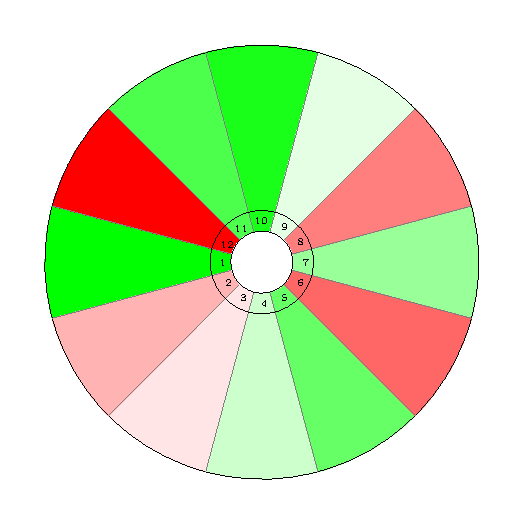
\includegraphics[width=0.7\textwidth]{diagrams/superior-places}
\vspace{-1em}
\caption{The Superior Places}
\end{figure}
\begin{mdframed}[backgroundcolor=cyan!5, rightmargin=1em, leftmargin=1em]
\small
In the figure the seven \textsl{good} places are in shades of green; the bad in shades of red.
\end{mdframed}
\section{Power of the Seven Planets}

Every planet in its own sign, exaltation, or triplicity is benefic as ``what it indicates of good is strong, increasing.'' This is true even of malefics as their ``evil becomes lighter and decreases'' when they are in their own places.

\Saturn\, in a masculine sign\footnote{In \S1.4 we are told \Saturn\,(a diurnal planet) is at his worst when in a feminine sign. Here we are told he can still do harm when in a masculine sign but not as much and even less if he is in one of his own dignities. In the same section, \Mars\, (a nocturnal planet) in a feminine sign is described as less harmful than a feminized \Saturn.} in a day chart (even though he is a diurnal planet) can cause harm but it will be less harmful if he is also in one of his own dignities. The same is true for \Mars, a nocturnal planet, in a feminine sign in a nocturnal chart. 

A planet's power \textsl{disappears} if it is within 15° of the \Sun\, while the \Sun\, is moving towards a conjunction with the planet.

A retrograde planet indicates ``there is difficulty [and] misfortune'' for the person and others.


\section{More on Upbringing}

\subsection{Good Upbringing}
\label{sec:upbringing2}
The person will be brought up if diurnal planets in a diurnal chart or nocturnal planets in a nocturnal chart are found in:
\begin{itemize}[topsep=0pt,itemsep=0pt]
\item one or more of the seven strong places; it is beneficial if one of them is a benefic

\item the 2nd place from the ascending sign if the planet is within 15° of the Ascendant as then ``reckon its power as if it were in the ascendent''
\end{itemize}

\subsection{No Upbringing}
The person may not be brought up or have a harsh upbringing if:
\begin{itemize}[topsep=0pt,itemsep=0pt]
\item the first triplicity ruler is within 15° of the \Sun\, or in a bad place; especially if the second triplicity ruler is with him

\item both malefics aspect the \Moon, especially if she is in an angle and one of the malefics is in opposition while also making an exact aspect to the Ascendant\footnote{Dykes indicates it could be an aspect to the Ascendant's terms rather an exact aspect to the Ascendant's degree (CAD p.69).} as ``this is an indications of ruin''

\item the \Moon\, in the 7th place with no connection to a benefic and while a malefic is in an angle for ``then the women give birth to what has no escape from ruin''

\item the \Moon, not in her own places, in the 4th with \Saturn\, and \Mars\, or in their opposition

\item one of the malefics in the Ascendant opposite the other malefic and the \Moon\, in the 10th or 7th

\end{itemize}

\subsection{Rejection or Exposure}
The person may be cast out by his parents if:
\begin{itemize}
\item the \Moon\, in the 4th place with \Saturn\, and \Mars\, or in their opposition unless the \Moon\, is in her own triplicity and the benefics are trine the malefics in which case, rather than ruin, the person is brought up by strangers and sometimes they ``will be a slav and will be employed and then will be miserable''

\item the \Moon\, ``between the two malefics and one them casts its rays upon it'' then the person's livelihood will be little and if the \Moon\, is also waning ``it indicates fate and shortness of life'' which he may escape if a benefic is also part of the configuration

\item the \Moon\, is with a malefic in an angular or succedent place and is configured with a benefic and if the \Sun\, aspects the malefics, the father favours casting him out and thinks badly of him; if the \Moon\, is injured\footnote{This is odd as we've already been told the \Moon\, must be with a malefic, which would be an injury; possibly it must also be harmed by the other malefic?}, the mother wants to cast the person out; if both lights are injured, both parents want rid of the person

\item in a diurnal chart, \Mars\, angular and opposing the \Moon\, or the \Sun\, while they are not in their own places; in a nocturnal chart, \Saturn\, under the same conditions
\end{itemize}

\subsection{Calamity}

If the \Moon\, is in the term of a malefic without the aspect of a benefic while a malefic is in an angle there is ``calamity'' for the person unless first ruler of the sect light's triplcity aspects the \Moon.

\subsection{Injury to the person and his mother}

If there is no benefic in (a) an angle, (b) in the same sign as the Lot of Fortune, or (c) in a sign of the same triplicity as the Ascendant while malefics aspect the \Sun, \Moon, and SAN\footnote{The most recent new or full moon that occurred prior to the birth.} the indications are evil.

If a benefic does not aspect the Ascendant (representing the person) or the \Moon, an unfortunate condition is indicated for the person and their mother if the \Moon, or worse yet, the \Moon\, and \Venus\, (as both indicate the mother) are injured.

\textsl{\small(also see \S\ref{sec:upbringing} Upbringing and \S\ref{sec:upbringing3} Upbringing Again, \S\ref{sec:upbringing4} Upbringing and Livelihood)}

\newpage